\chapter{Литературный обзор}
\label{chap:theory}

% Общая информация о МЕМС датчиках
\section{Общая информация о микромеханических датчиках}
\label{sec:general_info_nt}

Микромеханические датчики (микроэлектромеханические системы, МЭМС) — это миниатюрные устройства, которые сочетают механические элементы и электронные схемы. Размеры компонентов таких датчиков варьируются от 1 до 100 микрометров, а самих устройств — от нескольких миллиметров до нескольких сантиметров \cite{adams_layton_2010}.


МЭМС-устройства обычно изготавливают на кремниевой подложке с помощью технологии микрообработки, аналогично технологии изготовления однокристальных интегральных микросхем \cite{adams_layton_2010}.

В основе их работы лежат различные физические законы, благодаря которым можно преобразовать различные механические воздействия в электрический сигнал и наоборот.


МЭМС (микроэлектромеханические системы) датчики широко применяются в различных отраслях благодаря их миниатюрным размерам, низкому энергопотреблению и высокой точности. В качестве основных областей применения можно выделить:

\begin{itemize}
	\item бытовая электроника;
	\item промышленность;
	\item медицина и биотехнологии;
	\item энергетика;
\end{itemize}

Для МЕМС датчиков бытового назначения основным требованием является высокая энергоэфективность, малые габаритные размеры, а также низкая стоимость производства. В то же время, датчики, которые используются в более высокоточных системах должны обладать низкими шумовыми характеристики и высокой чувствительностью.

\newpage

% Теоретическое описание работы акселерометров
\section{Устройство акселерометра}

Акселерометр — прибор, измеряющий проекцию кажущегося ускорения (разности между истинным ускорением объекта и гравитационным ускорением) \cite{habr_mems}. Они широко применяются в смартфонах, автомобилях, промышленности и медицинских устройствах благодаря своей компактности, низкой стоимости и высокой точности.

МЭМС-акселерометр состоит из подвижной массы (инерционного элемента), закрепленной на упругих подвесах, и неподвижных электродов. При ускорении масса смещается, что приводит к изменению ёмкости или пьезоэлектрического сигнала, который преобразуется в электрический сигнал.

\begin{figure}[ht]
	\centering
	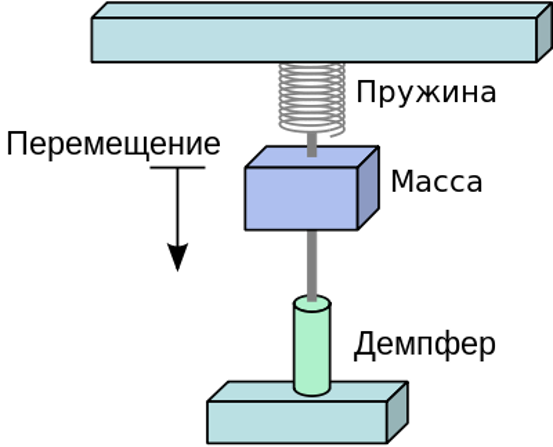
\includegraphics[width=0.5\textwidth]{images/theory/акселерометры/Схема работы акселерометра.png}
	\caption{Схема работы акселерометра}
\end{figure}

Основные методы измерения:

\begin{itemize}[label=$\circ$]
	\item Пьезоэлектрический
	\item Ёмкостный
	\item Тензорезисторный
\end{itemize}
\newpage
\subsection{Пьезоэлектрические акселерометры}


Пьезоэлектрический метод измерения основан на использовании прямого пьезоэффекта.
Прямое пьезоэффект - явление возникновения на поверхности пьезоэлектрика за счёт электрической поляризации под действием механического напряжения.
В качестве пьезоэлектриков используются анизатропные кристаллы естественного происхождения (например \ce{SiO2}), синтетические кристаллы (сегнетова соль \ce{C4H12KNaO10}) и поляризованные поликристаллические сегнетоэлектрики (пьезокерамика).

Для описания механического напряжения используют тензор напряжений.

\begin{figure}[ht]
	\centering
	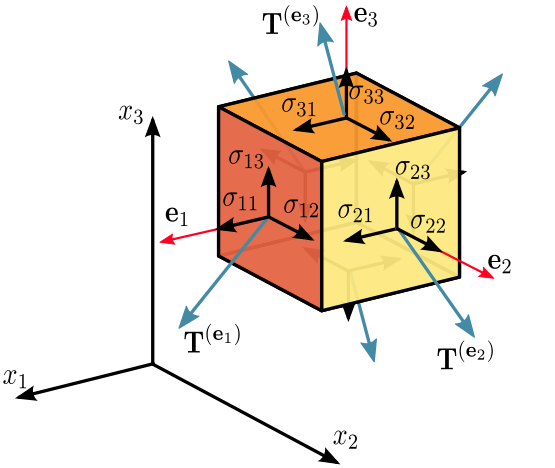
\includegraphics[width=0.5\textwidth]{images/theory/акселерометры/Тензор напряжений.png}
	\caption{Тензор напряжений}
\end{figure}

$
\mathbf{T} = 
\begin{bmatrix}
	\sigma_{11} & \tau_{12} & \tau_{13} \\
	\tau_{21} & \sigma_{22} & \tau_{23} \\
	\tau_{31} & \tau_{32} & \sigma_{33}
\end{bmatrix} = 
\begin{bmatrix}
	T_{11} & T_{12} & T_{13} \\
	T_{21} & T_{22} & T_{23} \\
	T_{31} & T_{32} & T_{33}
\end{bmatrix} = (T_{1}, T_{2}, T_{3}, T_{4}, T_{5}, T_{6})
$ \\

Одно из уравнений прямого пьезоэффекта, связывающее напряжение электрического поля и компоненты тензора механических деформаций:
\begin{equation}
	E_{i} = g_{ik} * T_{k}
\end{equation}
где $g_{ik}$ - пьезоконстанта давления.
\newpage

\subsection{Ёмкостные акселерометры}
Принцип работы ёмкостных акселерометров основан на изменении емкости конденсаторов при изменении ускорения.

\begin{figure}[ht]
	\centering
	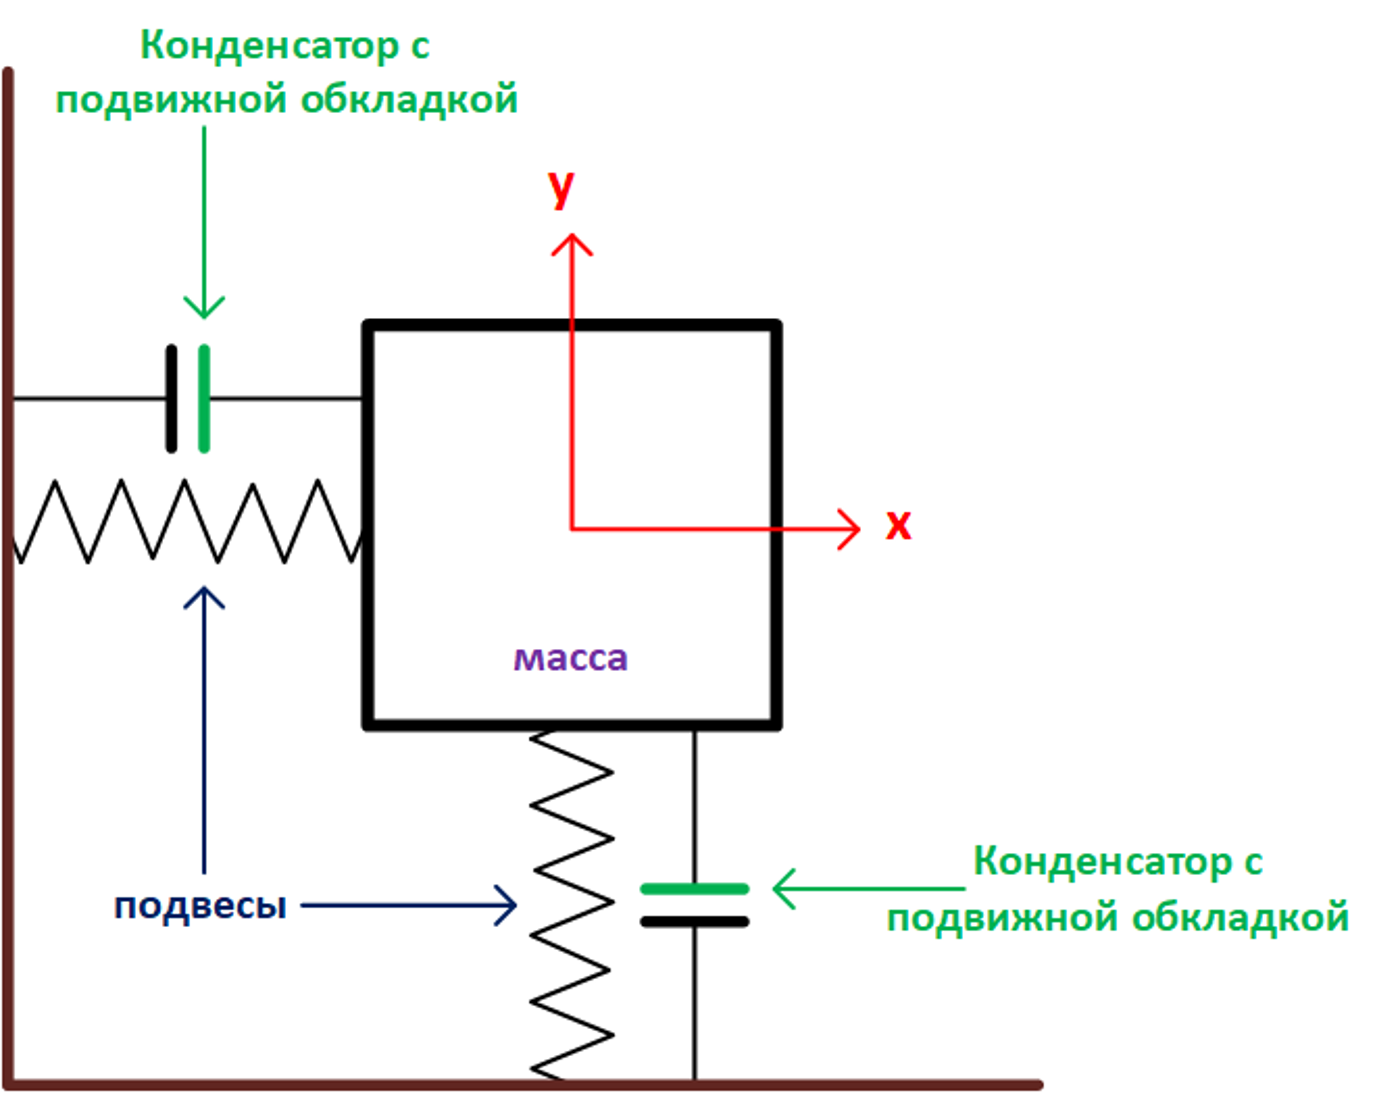
\includegraphics[width=0.55\textwidth]{images/theory/акселерометры/Схема ёмкостного акселерометра.png}
	\caption{Простейшая схема ёмкостного акселерометра}
\end{figure}

При изменении ускорения, масса изменяет расстояние между обкладками конденсатора. Из простейшей формулы емкости конденасатора $C=\frac{\varepsilon\varepsilon_0S}{d} $ следует, что при изменении d расстояния между обкладками емкость конденсатора будет также изменяться. \\ 

\begin{figure}[ht]
	\centering
	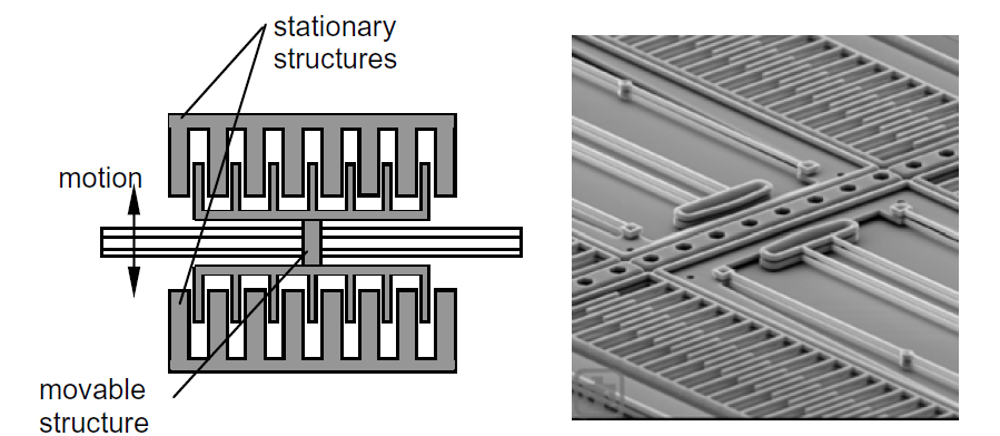
\includegraphics[width=0.7\textwidth]{images/theory/акселерометры/Изображение ёмкостного датчика.png}
	\caption{Устройство ёмкостного акселерометра, выполненного на кремниевой подложке}
\end{figure}

Изменение ёмкости превращается в сигнал с помощью довольно распространённой схемы - ёмкостной полумост.

\begin{figure}[ht]
	\centering
	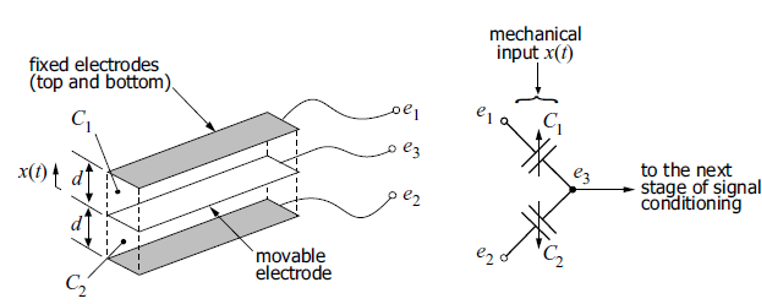
\includegraphics[width=0.7\textwidth]{images/theory/акселерометры/Схема ёмкостного полумоста.png}
	\caption{Схема ёмкостного полумоста}
\end{figure}

Напряжения $e_1$ и $e_2$ являются входными, а $e_3$ – выходной сигнал для последующего преобразования. Емкости обоих конденсаторов зависят от внешнего ускорения, и изменяются на величину x(t). При x = 0, заряды на емкостях являются идентичными, и при этом $C_1=C_2=C_0$. При условии, что x << d найдем как зависит изменение емкости конденсаторов от изменения положения обкладки.

Запишем изменение каждой емкости при сдвиге обкладки на x:
\begin{equation*}
	\Delta C_1=C_1-C_0 \ \ \ \ \ \ \ \ \ \ \ \ \ \  
	\Delta C_2=-C_2+C_0
\end{equation*}


Запишем через формулу емкости:
\begin{equation*}
	\Delta C_1=\frac{\varepsilon S}{d-x}-\frac{\varepsilon S}{d} \ \ \ \ \ \ \ \ \ \ \ \ \ \ \
	\Delta C_2=-\frac{\varepsilon S}{d+x}+\frac{\varepsilon S}{d}
\end{equation*}


Упростим данные формулы и учтём, что x << d. Тогда получим формулу изменения емкости конденсатора, в зависимости от смещения обкладки:
\begin{equation*}
	\Delta C_1=\frac{\varepsilon Sx}{d^2-xd}; \ \ \ \ \ \ 
	\Delta C_2=\frac{\varepsilon Sx}{d^2+xd} \\
\end{equation*}

\begin{equation}
	\Delta C\left(x\right)=\frac{\varepsilon S}{d^2}x
\end{equation}

\hspace{0.5cm}

Вводём дополнительные токи — $i_1, i_2, i_3$. По первому закону Киргофа получаем $i_1 + i_2 = i_3$ \\ 
Учитывая тот факт, что ток является производной заряда $i = \frac{dq}{dt}$ и заряд \ \ $q=CU$, получаем при $e_1=e_s$, а $e_2=-e_s$ зависимость выходного тока:

\begin{equation}
	i_{3} = 2 \left( e_{s} \frac{\epsilon S}{d^2} \dot{x} + x \frac{\epsilon S}{d^2} \dot{e_{s}} - C_{0}\dot{e_{s}} \right) 
\end{equation}

\newpage
%\subsection{Тензорезисторные датчики}
Их работа основана на тензоэффекте: изменение электрического сопротивления тензорезистора при его деформации. 

\begin{equation}
	K = \frac{\sfrac{\Delta R}{R}}{\epsilon}
\end{equation}
- коэффициент относительной тензочувствительности.

\begin{equation}
	\frac{\Delta R}{R} = \frac{\Delta \rho}{\rho} + \frac{\Delta l}{l} - \frac{\Delta S}{S} = \frac{\Delta \rho}{\rho} + \frac{\Delta l}{l} - \frac{2\Delta r}{r} = \frac{\Delta \rho}{\rho} + (1 + 2\mu)\epsilon
\end{equation}

где $\mu$ - коэффициент Пуассона. Первое слагаемое - физическая тензочувствиельность, а второе - геометрическая тензочувствительность. 

Для металлических проводников 

\begin{equation}
	\Delta \rho = \rho [\pi_{11} \sigma_{1} + \pi_{12}(\sigma_{2} + \sigma_{3})]
\end{equation}
где $\sigma_{123}$ - компоненты нормальных напряжений, $\pi_{11} \ pi_{12}$ - тензорезистивные коэффициенты.

При линейных напряжениях $\sigma_{1} = \sigma, \ \sigma_{2} = \sigma_{3} = 0$.
Откуда

\begin{equation}
	\frac{\Delta \rho}{\rho} = \pi_{11} \sigma = \pi_{11}E\epsilon    
\end{equation}
где Е - модуль Юнга.

\newpage
\newpage

% Теоретическое описание работы гироскопов
\section{Гироскопы: классификация и физические принципы работы}
\label{sec:gyroscope}

Гироскоп — это устройство или прибор, способный измерять изменение углов ориентации связанного с ним тела либо самостоятельно определять и сохранять заданное направление в пространстве. В основе работы большинства гироскопов лежит фундаментальное свойство вращающегося тела — сохранение направления оси своего вращения при отсутствии воздействия внешних моментов сил \cite{babaeva1973giroskopy}.


Общая классификация гироскопов может быть проведена по различным признакам: по физическому принципу действия, функциональному назначению, уровню точности, конструктивному исполнению. Наиболее фундаментальной является классификация по физическому принципу действия, которая отражает эволюцию технологии:

\begin{itemize}
	\item Механические гироскопы (роторные).
	\item Оптические гироскопы (лазерные, волоконно-оптические).
	\item Вибрационные гироскопы (МЭМС, кварцевые).
\end{itemize}






\subsection{Механические гироскопы}

Работа механических гироскопов базируется на законах механики вращательного движения твердого тела, в частности, на законе сохранения кинетического момента \cite{babaeva1973giroskopy}.

Гироскопический эффект проявляется в двух основных свойствах:

\begin{enumerate}
	\item Свойство инерциальности (устойчивости): Быстро вращающийся ротор (маховик) с большим кинетическим моментом стремится сохранить неизменным направление своей оси вращения в инерциальном пространстве.
	\item Свойство прецессии: При действии на гироскоп внешнего момента силы $\vec{M}$ его ось вращения совершает движение не в направлении действия момента, а в направлении, ему перпендикулярном. 
\end{enumerate}



\subsubsection{Конструктивные разновидности и особенности}

\begin{itemize}
	\item Гироскоп в кардановом подвесе (трехстепенной): Классическая конструкция, где ротор помещен в систему из двух или трех рам, изолирующих его ось от поворотов основания. Обеспечивает прямое измерение углов, но имеет существенные недостатки: трение в осях подвеса, ограниченный угол поворота рам, сложность конструкции.
	
	\item Динамически настраиваемый гироскоп (ДНГ): Ротор вращается внутри вращающегося карданова подвеса. При определенном соотношении скоростей («условии настройки») момент сил инерции, действующих на рамки, уравновешивается, и гироскоп становится астатическим. ДНГ не имеет ограничений по углу поворота, но требует сложной системы управления.
	
	\item Поплавковый интегрирующий гироскоп: Чувствительный элемент (ротор в подвесе) помещен в герметичный поплавок, который плавает в высокоплотной жидкости. Это обеспечивает гидростатическую разгрузку осей, демпфирование колебаний и термостабилизацию.
\end{itemize}

Исторически механические гироскопы являются основой инерциальной навигационной системы в авиации, ракетостроении и космонавтике. В настоящее время практически полностью вытеснены оптическими системами, за исключением некоторых специальных применений (например, гиростабилизаторы).

К достоинствам можно отнести высокую теоретическую и практическую точность у поплавковых моделей, прямое измерение углов ориентации и высокую надёжность в условиях специфических воздействий таким как перегрузки, радиация и электромагнитные импульсы.

Из недостатков можно упомянуть дрейф гироскопа из-за трения подвижных частей, большие габариты и вес готовой конструкции, а также ограничения по углам поворота гироскопа.


\subsection{Оптические гироскопы}

Оптические гироскопы не имеют подвижных механических частей в традиционном понимании. Их работа основана на явлении интерференции электромагнитных волн и эффекте Саньяка \cite{malkin_2002}.

Эффект Саньяка заключается в следующем: два когерентных луча света, распространяющиеся по одному и тому же замкнутому оптическому контуру в противоположных направлениях, приобретают разность фаз $\Delta \Phi$ при вращении контура с угловой скоростью $\Omega$:

\begin{equation}
	\Delta \Phi = \frac{8 \pi S}{\lambda c} \Omega
\end{equation}

где S — площадь, охватываемая контуром, $\lambda$ - длина волны света, c — скорость света.

% -----------------------------------------------------------------------------

\subsubsection{Лазерный гироскоп}

Конструктивные особенности лазерного гироскопа определяются необходимостью создания сверхстабильного кольцевого лазерного резонатора: его основу составляет цельный монолитный блок из сверхстабильной стеклокерамики (например, Церодур), в котором фрезерованы каналы, образующие замкнутый треугольный или квадратный контур. В углах резонатора установлены высокоточные многослойные диэлектрические зеркала, формирующие кольцевой оптический контур, причём одно из зеркал является полупрозрачным для вывода излучения на фотодетектор \cite{opticheskie_giroskopy_2005}. 

При вращении гироскопа резонансные частоты для встречных волн становятся разными. Возникает разность частот $\Delta f$ (частотный сдвиг Саньяка \cite{malkin_2002}), которая строго пропорциональна угловой скорости вращения $\Omega$. 

\begin{equation}
	\Delta f = \frac{4 S}{\lambda L} \Omega
\end{equation}

где L - периметр контура.

Таким образом, измеряя разность частот $\Delta f$, можно напрямую и с высокой точностью определить угловую скорость $\Omega$.

% -----------------------------------------------------------------------------

\subsubsection{Волоконно-оптический гироскоп}

Волоконно-оптический гироскоп — это тип оптического гироскопа, в котором для усиления эффекта Саньяка используется многовитковая катушка из оптического волокна \cite{volokonno_opticheskiy_1987}. Это пассивный интерферометрический прибор, ставший основной альтернативой и конкурентом лазерного гироскопа благодаря своей конструктивной простоте и высокой надежности.

Свет от внешнего широкополосного источника разделяется надвое, и два луча запускаются в противоположных направлениях в одну и ту же волоконную катушку. После прохождения контура лучи снова сводятся и интерферируют.

При вращении гироскопа возникает разность фаз $\Delta \Phi$ между встречными лучами, которая регистрируется фотодетектором \cite{volokonno_opticheskiy_1987}:

\begin{equation}
	\Delta \Phi = \frac{2 \pi L D}{\lambda c} \Omega
\end{equation}

где L — длина волокна, D — диаметр катушки, $\lambda$ — длина волны света, c — скорость света, $\Omega$ — угловая скорость.

Ключевой конструктивной особенностью волоконно-оптического гироскопа является его модульная структура, центральным элементом которой служит многовитковая катушка (длиной от сотен метров до нескольких километров) из одномодового, сохраняющего поляризацию оптического волокна, намотанная особым способом для минимизации температурных и вибрационных помех. Весь оптический тракт формируется вокруг интегрально-оптического чипа, выполняющего функции разделителя, поляризатора и фазового модулятора, а в качестве источника излучения используется широкополосный суперлюминесцентный диод для подавления паразитных интерференционных шумов.


\subsection{Вибрационные гироскопы}

Вибрационные гироскопы представляют собой класс инерциальных датчиков, в которых для измерения угловой скорости используется не вращение постоянного ротора, а колебательное движение (вибрация) чувствительного элемента \cite{mems_sensors}. Их развитие, особенно в области микроэлектромеханических систем (МЭМС), совершило революцию, сделав гироскопические технологии массовыми и доступными.

Для корректного анализа работы вибрационных гироскопов, в частности МЭМС-датчиков угловой скорости, необходимо строгое рассмотрение кинематики движения в неинерциальных системах отсчёта, задаваемое теоремой Кориолиса \cite{persson2005coriolis}.

% -----------------------------------------------------------------------------

\subsubsection{Теорема Кориолиса}

Рассмотрим движение материальной точки в двух системах координат: инерциальной системе OXYZ и неинерциальной системе Ox'y'z', которая вращается относительно инерциальной с мгновенной угловой скоростью $\vec{\omega}$.

Тогда абсолютная скорость рассматриваемой материальной точки будет по теореме сложения скоростей будет равна:

\begin{equation}
	\vec{v} = \vec{v_{0}} + [\vec{\omega}, \vec{R}] + \vec{v_{r}}
\end{equation}

где $\vec{R}$ - радиус-вектор точки относительно мгновенного центра скоростей 
O, $\vec{V_{0}}$ - переносная скорость точки, $\vec{V_{r}}$ - её относительная скорость.

Продифференцируем это равенство по времени:

\begin{equation}
	\frac{d}{dt} \vec{v} = \frac{d}{dt} \vec{v}_0 + \frac{d}{dt} \left[ \vec{\omega} \times \vec{R} \right] + \frac{d}{dt} \vec{v}_r.
\end{equation}


Найдём значение каждого слагаемого в инерциальной системе координат:

\[
\frac{d}{dt} \vec{v}_0 = {\vec{a}}_0,
\]

\[
\frac{d}{dt} \left[ \vec{\omega} \times \vec{R} \right] = \left[ \vec{\varepsilon} \times \vec{R} \right] + \left[ \vec{\omega} \times \frac{d}{dt} \vec{R} \right] = \left[ \vec{\varepsilon} \times \vec{R} \right] + \left[ \vec{\omega} \times \left[ \vec{\omega} \times \vec{R} \right] \right] + \left[ \vec{\omega} \times \vec{v}_r \right],
\]

\[
\frac{d}{dt} \vec{v}_r = \left[ \vec{\omega} \times \vec{v}_r \right] + \frac{d_r \vec{v}_r}{dt},
\]

где \(\vec{a}_r\) — линейное ускорение точки относительно системы \(Ox'y'z'\), \(\vec{\varepsilon} = \frac{d\vec{\omega}}{dt}\) — угловое ускорение системы \(Ox'y'z'\).

Таким образом, имеем:

\[
\frac{d}{dt} \vec{v} = \ddot{\vec{a}}_0 + \left[ \vec{\varepsilon} \times \vec{R} \right] + \left[ \vec{\omega} \times \left[ \vec{\omega} \times \vec{R} \right] \right] + \ddot{\vec{a}}_r + 2 \left[ \vec{\omega} \times \vec{v}_r \right].
\]

\hspace{1cm}

Полученное равенство служит математическим выражением теоремы Кориолиса: Абсолютное ускорение точки в сложном движении равно геометрической сумме её переносного ускорения, относительного ускорения и добавочного кориолисова ускорения, равного \(2 \left[ \vec{\omega} \times \vec{v}_r \right]\).


При переходе к уравнению движения во вращающейся системе отсчёта это ускорение, взятое с обратным знаком и умноженное на массу точки, интерпретируется как сила инерции Кориолиса:

\begin{equation}
	F_{c} = -m · a_{c} = -2m [\vec{\omega}, \vec{v_{r}}].
\end{equation}

\vspace{0.5cm}

\begin{figure}[ht]
	\centering
	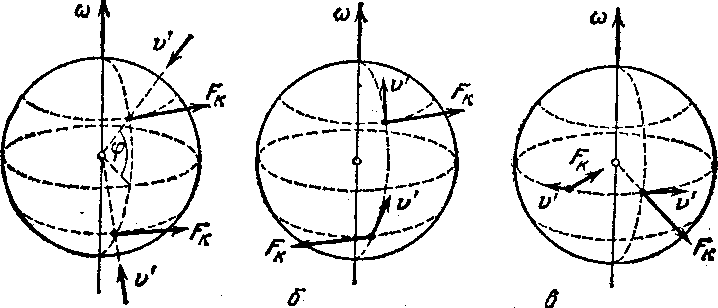
\includegraphics[width=0.7\textwidth]{images/theory/гироскопы/иллюстрация силы Кориолиса.png}
	\caption{Иллюстрация силы Кориолиса}
\end{figure}

В контексте вибрационных гироскопов $v_{r}$ — это скорость контролируемого колебательного движения чувствительной массы (режим привода), а $\omega$ — измеряемая угловая скорость корпуса прибора. Возникающая при этом сила Кориолиса $F_{c}$ вызывает вторичные колебания массы в перпендикулярном направлении (режим считывания), амплитуда которых пропорциональна $\omega$. Следовательно, теорема Кориолиса предоставляет фундаментальную физико-математическую основу для преобразования измеряемого вращения в измеримое механическое перемещение, что является ключевым принципом действия всего класса вибрационных гироскопических датчиков.

% -----------------------------------------------------------------------------

\subsubsection{Одноосевой МЕМС-гироскоп с вибрирующим кремниевым кольцом}

Описываемые гироскопы относятся к классу вибрационных твердотельных датчиков и характеризуются отсутствием классических вращающихся масс или подшипников. Единственным подвижным элементом является упругое сенсорное кольцо из монокристаллического кремния, совершающее микроскопические колебания, что обеспечивает исключительную долговечность и стойкость к механическим нагрузкам.

Принцип действия основан на измерении вызванной силой Кориолиса прецессии стоячей волны в резонаторе, что позволяет определять величину и направление приложенной угловой скорости \cite{mems_sensors}.

Ключевые элементы конструкции и режимы работы:

\begin{itemize}
	\item Чувствительный элемент: Кольцевой резонатор, подвешенный на упругих спицах или непосредственно на центральном основании.
	\item Система возбуждения и контроля первичной моды: По периметру кольца симметрично расположены восемь преобразователей. Одна пара выполняет роль приводов первичного движения, другая — первичных считывающих преобразователей. Они расположены на главных ортогональных осях, образуя замкнутую систему автоматического регулирования с ASIC-контроллером. Эта система возбуждает и поддерживает стабильные резонансные колебания первичной моды с частотой около 22 кГц. В этом состоянии кольцо деформируется, принимая квазиэллиптическую форму.
	\item Система считывания вторичной моды: Две дополнительные пары вторичных считывающих преобразователей расположены по осям, смещенным на 45° относительно главных. При отсутствии вращения радиальное движение в этих точках отсутствует.
\end{itemize}


\begin{figure}[ht]
	\centering
	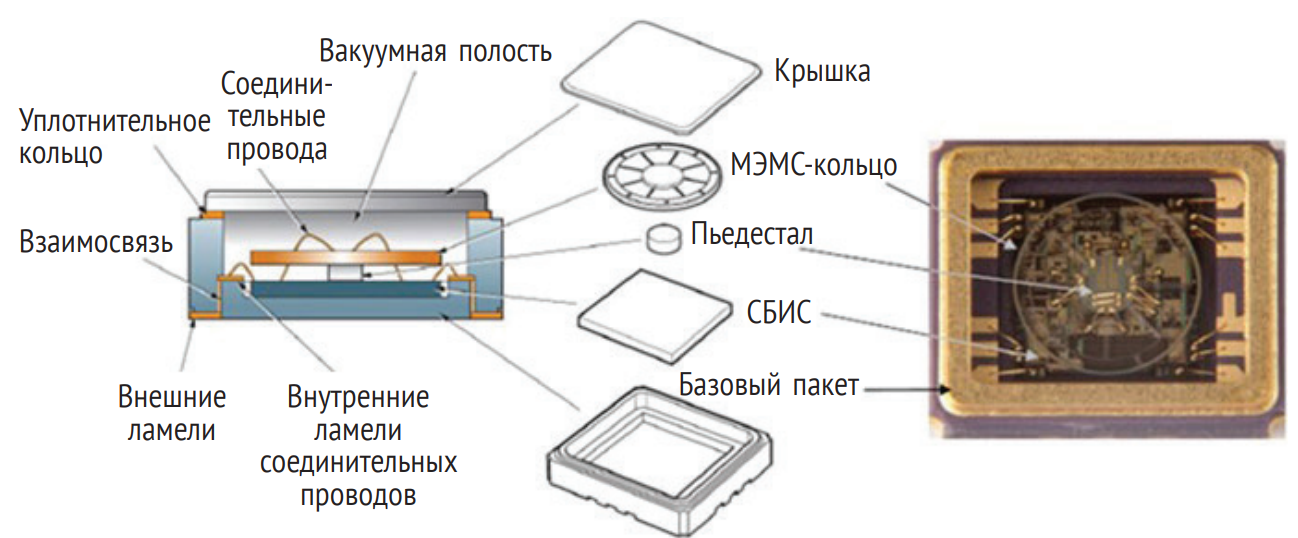
\includegraphics[width=0.9\textwidth]{images/theory/гироскопы/основные детали кремниевого гироскопа.png}
	\caption{Основные детали кремниевого гироскопа}
\end{figure}


\subsubsection{Принцип измерения угловой скорости}

Когда гироскоп начинает вращаться с угловой скоростью $\Omega$, на колеблющиеся участки кольца действуют силы Кориолиса. Эти силы, распределенные по периметру, не совпадают по фазе с первичными колебаниями и вызывают возбуждение вторичной (квадратурной) моды колебаний. Это приводит к прецессии узловой картины стоячей волны вокруг оси кольца. В результате на электродах вторичного считывания возникает сигнал радиального смещения, строго пропорциональный приложенной угловой скорости \cite{mems_sensors}.



\begin{figure}[H]
	\centering
	\begin{subfigure}{0.48\textwidth}
		\centering
		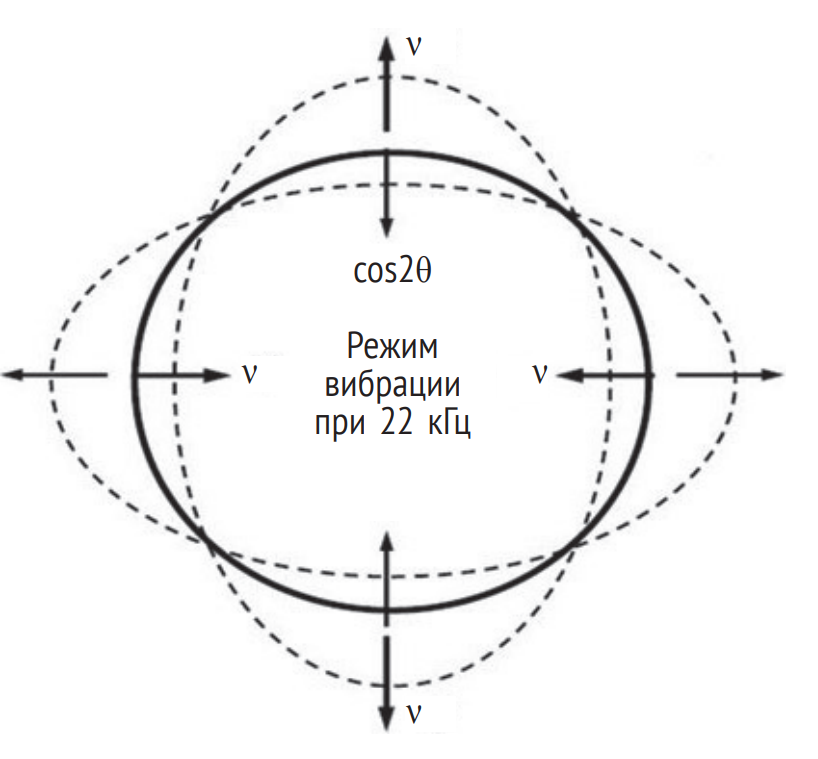
\includegraphics[width=0.7\textwidth]{images/theory/гироскопы/иллюстрация кольца в покое.png}
		\caption{Иллюстрация кольца \\ в состоянии покоя}
	\end{subfigure}
	\hfill
	\begin{subfigure}{0.48\textwidth}
		\centering
		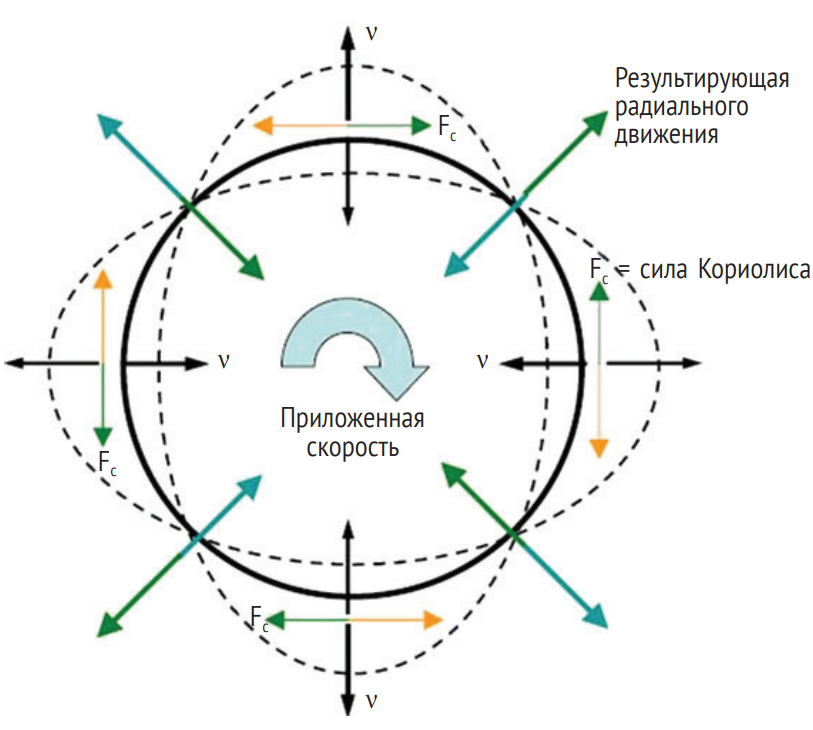
\includegraphics[width=0.7\textwidth]{images/theory/гироскопы/состояние гироскопа без движения.png}
		\caption{Иллюстрация состояния включенного гироскопа в отсутствие движения}
	\end{subfigure}
	\caption{Иллюстрации состояний вибрирующего кольца}
\end{figure}










% Обзор аналогов
\section{Обзор аналогов}

Обзор аналогов